\chapter{Introduction} \label{cha:introduction}
This chapter offers an overview of the project on which the thesis is based. The goal is to explain in detail how the practical problem has been approached in order to analyse the physical constraints, ideate a software method able to solve them, and how these ideas were then implemented into a working algorithm. 


\section{Physical context}
The physical component in this project is a robot. Its definition can vary a lot basing on the context in which it is used. For this project, a robot can be described as a vehicle able to move in the space. A \textbf{LIDAR (Laser Imaging Detection And Ranging)} sensor is mounted. Which allows to drive in the space avoiding physical obstacles during the movement. In addition, it is installed a computational device connected to a webcam that can record streams of images representing the space in front of the robot itself. The robots that we are working with are shown in~\Cref{fig:robots}.\\
The video camera becomes the eye of the robot itself, and the captured video stream is used as the input of the algorithm working on the computational device. This computer can be composed of a \textbf{CPU (Central Processing Unit)} or more likely it is built with a \textbf{GPU (Graphics Processing Unit)} that can speed up parallelized computation, applied on the \textbf{DNNs (Deep Neural Networks)} used as the core of the algorithm. The software does not assume one component over the other, the only variation is in the performances: a GPU computation speed can be much higher than a CPU.\\
Instead, the output of the algorithm is a position composed of X and Y pixel coordinates calculated on a single frame captured from the webcam. This location can be then elaborated and, with the use of LIDAR sensor, the robot can estimate which is the 3D position of the element tracked from the software.\\
Finally, it moves to reach that position, in order to follow the tracked subject not only into the virtual space but also into the real environment.

\begin{figure}[!h]
	\centering
	\begin{subfigure}{0.44\textwidth}
		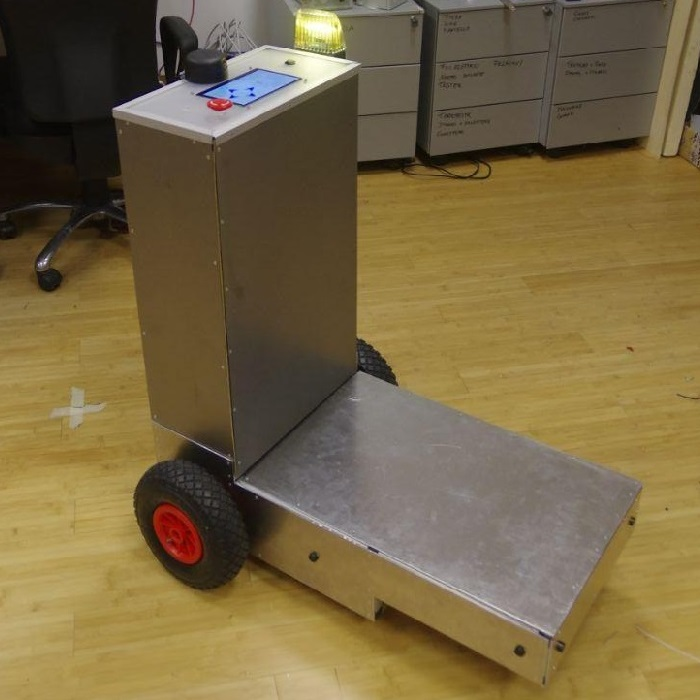
\includegraphics[width=\linewidth]{images/introduction/robot_shelfy}
		\captionsetup{margin=0.5cm}
		\caption{The first prototype designed to test applications that will be used in an industrial environment.}
	\end{subfigure}
	\begin{subfigure}{0.44\textwidth}
		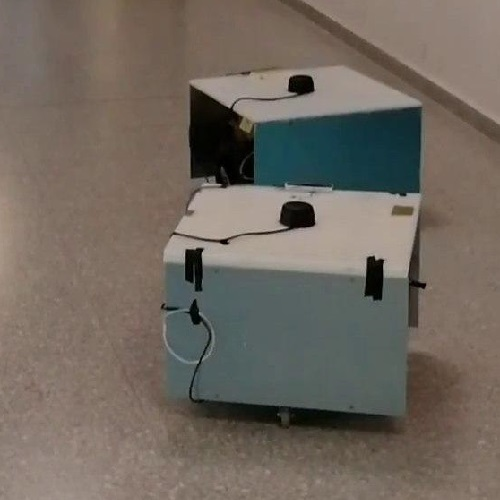
\includegraphics[width=\linewidth]{images/introduction/robot_shelfini}
		\captionsetup{margin=0.5cm}
		\caption{A small model designed to build a fleet of robots that interact with each other while moving.}
	\end{subfigure}
	\captionsetup{margin=0.5cm}
	\caption[Pictures of the robots used for this thesis.]{These are the two model of robots on top of which we have designed this thesis project. The two models share the same physical characteristics.}
	\label{fig:robots}
\end{figure}

\section{The problem}
The thesis project\cite{projectSourceCode} is based on an internship with Dolomiti Robotics\cite{dolomitiRobotics}, a company working on self-driving robots.\\
These vehicles are designed to work in an industrial environment. This scenario is populated not only by robots but also people, making the driving task even more complex to achieve.

\subsection{Robot only environment}
A completely automated environment, where humans cannot access looks to be a similar context. Instead, it is completely different because each vehicle has is its own logic that can be designed to fit the requirements of all the other robots working in that area.\\
The typical solutions to drive a vehicle in this scenario are two:
\begin{itemize}
	\item Based on a centralized decision unit that moves all the robots simultaneously around. This unit is responsible for avoiding collisions by knowing the exact position of each single moving robot.
	\item Based on fixed rules of movement that each robot has to follow. The rules do not allow collision and the automated vehicles respect them.
\end{itemize}
Both these methods work because an automated vehicle uses a deterministic decision process and does not take arbitrary choices.

\subsection{Environment shared between robots and humans}
Instead, in a shared environment, there are a lot of elements that are not controlled by a deterministic rule. The changes in the scenario are random and prediction cannot be done. There are both fixed object that may have changed position due to external interaction, and also human that walk around with no defined rules.\\
In this scenario, it is fundamental to choose an input method that can measure the area around, in order to create an autonomous moving vehicle. Therefore LIDAR has been chosen. LIDAR is a technology that measures distances around the robot in a horizontal plane. The effect is that the robot knows in each direction which is the distance from the surrounding objects. This key idea has been used from Dolomiti Robotics, to design a software able to drive robots around avoiding collision with fixed obstacles or people walking.\\
While a robot moves around, it can construct a map of the fixed objects in the environment, measured with LIDAR. Instead, the moving objects, such as other robots or people, that are recognised as not fixed elements are not stored in the map as obstacles. This reconstruction allows the vehicle to move autonomously from one position to another knowing exactly which path to follow to reach the destination.

\subsection{Purpose of the internship}
The shared environment does not offer any real human-robot exchange. The two parts only share the same spaces. The purpose of this thesis project is to create a physical interaction between the two.\\
The goal is to create a new functionality \textit{"that allows a robot to follow a person into the real environment"}. How it works:
\begin{itemize}
	\item Track/follow is the interaction of a robot and a single person (called from now on \textbf{leader}).
	\item The leader starts the \textit{"follow"} functionality standing in front of the webcam of the robot.
	\item The robot has few seconds to recognise the person inside the camera \textbf{FOV (Field Of View)} as the leader.
	\item Then the leader can freely move around in the space. 
	\item In the meanwhile the algorithm is processing the webcam stream of images recognising the position of the leader and start tracking it in the virtual space, while following it in the real one.
	\item The tracking continues for a long period, up to several minutes until this functionality is stopped.
\end{itemize}

\subsection{Technical problems}\label{sec:technicalProblems}
This "follow" functionality may be easily solved under certain conditions. However, solving the general scenario, it is a much harder task.\\
Below is listed a small collection of the principal problems that make this functionality an extremely general one, therefore hard to solve.
\begin{itemize}
	\item The tracking should be done in real-time. It is impossible to follow a person if the processing speed is too slow. A high \textbf{FPS (Frames Per Second)} rate should be respected.
	\item The robot needs to physically follow the person meaning that the webcam cannot be fixed. By consequence, also the background is not fixed and the entire captured image, subject included, might be blurred.
	\item The person can move freely around walking fast, slow, or staying.
	\item The leader is a random person, it is not known while the algorithm was designed (no parameters can be fixed in advance).
	\item While the leader is walking around there might be also other people that interfere with the algorithm.
	\item The leader can be hidden from the webcam due to moving or static elements placed between the leader and the webcam itself.
	\item The leader can exit the field of view of the webcam disappearing until the robot rotates to watch it back again.
	\item The tracking should be performed for a long period.
\end{itemize}


\section{The solution}
The problem is complex due to its generality and the necessity to cover a lot of complementary conditions. For this reason more than one solution exists. In this thesis is presented a solution based on the combination of three methods. Each one is designed to solve sub-problem compared to this one, and none of them alone can overcome the challenge of the general task.\\

\subsection{Existing technologies}\label{sec:existingTechnologies}
The three technologies are:
\begin{itemize}
	\item \textbf{Object Detection (or Localization):} given an image the object detection task aim at processing the image and recognise which objects exist there. The detection not only need to produce a list of all the classes\footnote{There are a set of types to which each element can be associated i.e. person, dog, car, bicycle, bottle and so on.} of objects visible in the image, but also recognise in which section of the frame every single element is.\\
	The output of detection is a list of: class to which the element belongs, the probability associated and the \textbf{bounding box} defined as the smallest rectangle that contains the entire element.

	\item \textbf{Object Tracking:} in this case the input is not a single image but a video stream and an initial section\footnote{A portion of the image: a rectangle.} of it. The goal is to remember this portion of the image and recognise it in all the frames after the first one. It is important to note that the tracking procedure it is not designed to follow a person, a car or other it is designed to follow a rectangle of coloured pixels, no matter what these pixels represent.

	\item \textbf{Object Recognition:} this is a comparison between several pictures. These often represent a bounding box of the object that needs to be recognised. The procedure has a database of images each one with a specific class, and the input value is another picture, called \textbf{query}, that does not exist in the database but it represents a subject known. The goal is to extract from the database all the images that have a subject that looks similar to the one represented in the query.\\
	This application is mainly used to recognise humans, often in the video surveillance context. The database is composed of the bounding box of all the people seen, i.e. in a supermarket over the last week, and when a thief is captured and it is used as a query. So, the system should return all the images containing the thief itself.
\end{itemize}

\subsection{Limitation of known technologies}
The challenges presented previously in \Cref{sec:existingTechnologies}, can solve a small part of the general problem but each one has a technical problem~\Cref{sec:technicalProblems} that cannot be solved:
\begin{itemize}
	\item Object detection is a computationally expensive task, on a powerful GPU can run in real-time but that is not the case of the robots we are working with.\\
	In addition, the detection works frame by frame and each one is independent of the previous one. So, if a person is recognised in a frame, and in the next one, there is more than a single person the algorithm does not know the relation between all of them. Meaning that a person cannot be tracked from one frame to the next one.

	\item Object tracking, according to the name, seems the task that better match the requirement of the general problem.\\
	Despite that, the tracking does not consider that the tracked subject, the leader, cannot be hidden from the webcam. The leader should always be visible into the recorded video, and that is not the case. In addition, the leader can also exit the field of view of the robot while walking around.\\
	Lastly, all the trackers are designed to follow the subject for small periods\footnote{Each tracker works on a video of few seconds.}, after a while the tracked rectangle of coloured pixel changes and the precision of the output is no more not guaranteed. This phenomenon is known as the \textbf{drift effect}, after a while the drift is so wide that the tracked cannot be trusted anymore.

	\item Object recognition due to its requirement was not designed at all to run in real-time. In fact, it is enough to run this procedure only when a query occurs, and that does not happen more than one every second.\\
	Except that, there is a more intrinsic problem with the recognition to approach the general problem. The procedure requires a query that can be the subject at the actual frame, but then it should work on a dataset composed of old frames and these are useless to solve the actual frame.\\
	In addition, this algorithm cannot be independent, because the input values are bounding boxes of people, but these regions can be computed only with an object detection algorithm. Hence this approach cannot solve the problem independently.
\end{itemize}

This explanation shows that none of the existing proposed technologies can solve the general problem in all its parts.

\subsection{Combine known methods to solve the general task}
To solve the problem and manage all the requirements it is necessary to create a combination of known methods.\\
An example of integration of methods to solve a complex task was done by Jiang et al, in their paper\cite{multi-feature-fusion-and-YOLO} that presents a fusion of \textbf{YOLO9000}\cite{yoloV2} (the second version of \textbf{YOLO}\cite{yolo}) used as object detector and \textbf{SURF}\cite{surf} used as short-term object tracker.\\
The paper illustrate an innovative approach based on two thresholds that are used to understand when the drift of the tracker is too large and it is necessary to reinitialize it. So YOLO is executed to find the tracked subject back again and after the initialization the loop can start again.\\
\\
The method presented in that paper is an integration of two class of methods. Instead in this thesis is presented an integration of three. The third method is necessary because an additional technical problem exists~(\Cref{sec:technicalProblems}). Jiang et al. work on sport video clips where athletes are always followed by the camera and never disappear out of the field of view. In addition, occlusion can exist but are very short and the tracker is often able to overcome them.\\
Instead, in our scenario we need  to manage the disappearance of the leader behind a corner for a relatively long time. So, the object recognition method was introduced to solve this condition.\\ 
These are the main steps of the entire algorithm:
\begin{enumerate}
	\item The \underline{detection} module is executed and the bounding box of the leader is found. By assumptions, in this phase, if more than one person is simultaneously found the leader is chosen according to the area of the bounding boxes. The biggest area represents the most important person hence the leader.\\
	This step is executed several time to train the people recognition module.
	\item A new detection is executed and D people are found.
	\item Ad hoc optimizations and the \underline{people recognition} module is used to choose if the leader is contained in the list of people found:
	\begin{itemize}
		\item If \textbf{yes}: the procedure starts from point 4 (tracking)
		\item If \textbf{not}: the procedure loops again from point 2 (detection again)
	\end{itemize}
	\item The \underline{tracker} module is initialized with the bounding box found.
	\item The tracker runs for the next F frames. When stopped loop back to point 2.	
\end{enumerate}

This flow shows how detection, tracking and recognition are combined together to build a complete algorithm, that can run in real-time due to the alternation of slow and fast methods and to manage all the problematic scenarios.\\
The details will follow.


\section{Prior technical knowledge}
In this section are presented some technologies that should be known in order to well understand the algorithms presented in the next chapters.

\subsection{NN (Neural Network)} \label{sec:nn}
A NN\footnote{A visual and very well done explanation on how a NN works can be found online. The 3Blue1Brown youtube channel has published videos about the mechanics of \href{https://www.youtube.com/watch?v=IHZwWFHWa-w}{gradient descent} and about the learning phase based on \href{https://www.youtube.com/watch?v=Ilg3gGewQ5U}{back-propagation}.} is a black box containing several layers (\Cref{fig:howItWorks_NNlayers}). Each layer takes as input the output values of the layer before. The input of the NN goes into the first layer and the output comes from the last one. Each layer is composed by a certain amount of neurons (\Cref{fig:howItWorks_neutron}). Each of these neurons computes a weighted summation of all the output values of the neurons in the previous layer. For each couple of neurons in consecutive layers exists a weight that multiplies the output of the first one to generate the input of the next one. The final output of a neuron is then computed by summing up a bias value and by applying an activation function such as ReLU (Rectified Linear Unit), SoftMax or Identity.

\subsubsection*{Gradient descend}
The final prediction of the NN corresponds to the label of the neuron, in the last layer, with the highest value. The overall output of the last layer is evaluated with a \textbf{cost function}. The higher the cost the worst were the prediction. A perfect prediction will have cost equal to zero. The general cost of a model is the average cost computed on the entire input training set.\\
The training of the NN is based on the minimization of the cost function. Since that the cost function is based on thousands of dimensions that represent the weights over the entire NN, the minimization cannot be analytically solved. The solution is the \textbf{gradient descend} technique. Basically, a set of input values, and all the associated outputs, produce a specific average cost. This generated value is a point of the cost function, and it has an associated gradient. The measure of the gradient tells us how to modify the weights in order to produce a lower cost on the same input training set. Hence how to improve the NN performances by descending the cost function along the steepest path to reach a local minimum\footnote{We are "only" interest into local minimum since to find the global minimum it is necessary to explore the entire cost function and this requires a huge amount of time.}.\\
Unfortunately, the generation of the gradient with analytics techniques is unfeasible. Therefore we need the \textbf{back-propagation} technique to measure it.

\subsubsection*{Back-propagation}
Essentially the gradient represents the direction of the steepest path to the local minimum of the function. Another interpretation is that the magnitude of gradient represent for each dimension how the associated weight is useful for the final output prediction. For each input of the NN the neurons in the last layer should be tuned to produce a cost equal to zero. The variation for each neuron, compared to the correct value, depends on all the parameters of its summation. Practically, the elements involved are the neuron's output of the second-last layer and the associated weights. These parameters are linked one after the other, up to the left-most layer (the first one).\\
Therefore the last layer parameters can be computed to generate the best possible score. This variation will then influence the previous layer and its weights, then the one before and so on and so forth up to the first layer. This is the key idea of the back-propagation.\\
Once plenty of input has been passed through the NN and the tuning have been performed a lot of times, the weights are finally calibrated. The result, defined as the combination of the NN architecture and its weights is the called \textbf{model}. In this thesis work, we have never built our model but we have always used pre-trained ones.

\begin{figure}[!h]
	\centering
	\begin{subfigure}{0.49\textwidth}
		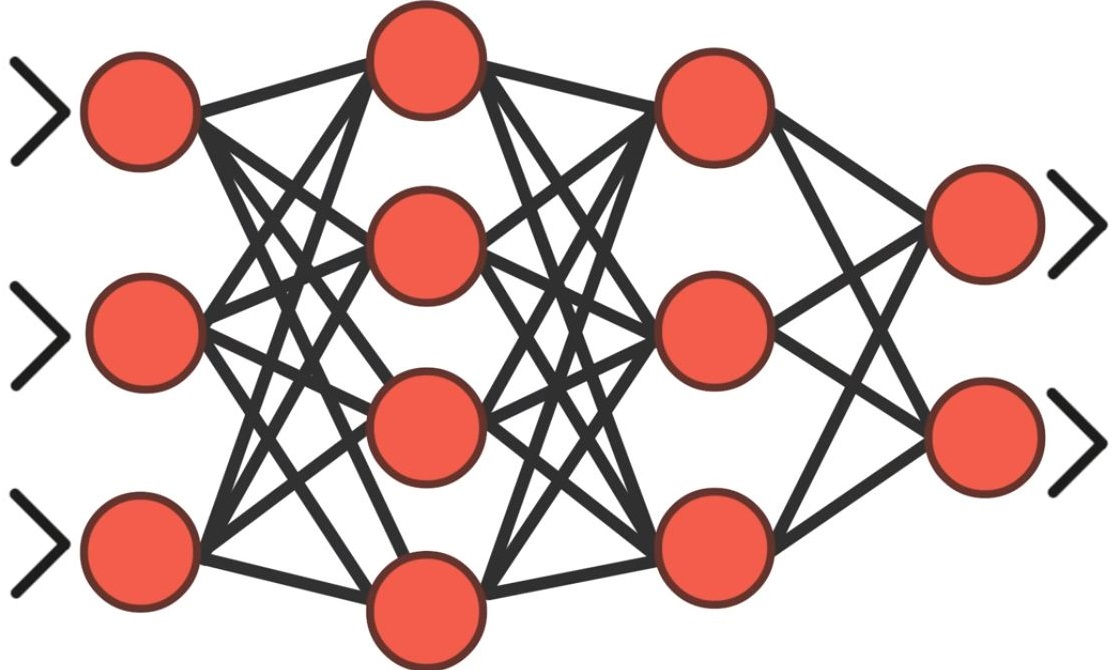
\includegraphics[width=\linewidth]{images/introduction/howItWorks_NN_layers}
		\captionsetup{margin=0.5cm}
		\caption{The general structure of a NN. The input, taken from the left, is passed through the four layers that generate the NN output on the right side. The four layers are respectively composed of 3, 4, 3 and 2 neurons.}
		\label{fig:howItWorks_NNlayers}
	\end{subfigure}
	\begin{subfigure}{0.49\textwidth}
		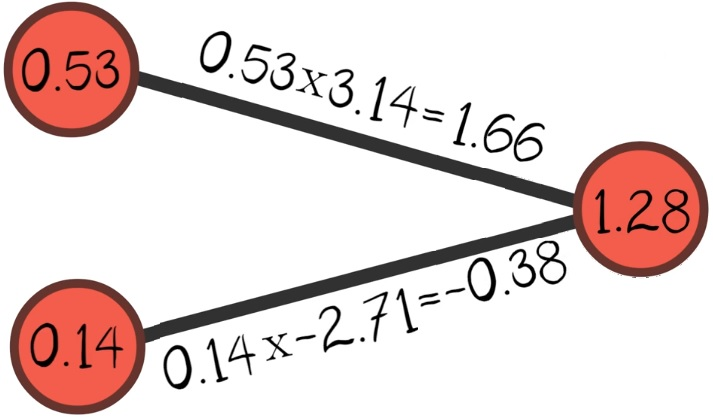
\includegraphics[width=\linewidth]{images/introduction/howItWorks_NN_neutron}
		\caption{The functioning scheme of a neuron. The outputs of the left-neurons are multiplied with ad hoc weights and then summed up. In addition, the right-neuron will add a bias value and apply an activation function to produce its output.}
		\label{fig:howItWorks_neutron}
	\end{subfigure}
	\captionsetup{margin=0.5cm}
	\caption{Two schemes that represent the key mechanics of a NN.}
	\label{fig:howItWorks_NN}
\end{figure}

\subsection{CNN (Convolutional Neural Network)} \label{sec:cnn}
A CNN\footnote{A visual explanation of the CNN, created by the DeepLizard youtube channel, is available \href{https://www.youtube.com/watch?v=YRhxdVk_sIs}{here}.}, also called \textbf{ConvNet}, is a standard NN extended to process images.\\
The novelty of this NN is characterized by a new type of layers: the \textbf{convolutional layers}. These layers are the main components of a CNN and are stacked one after the other. Often the end of the NN is composed of few traditional layers that compress the huge output of the previous layers, to generate the overall output of the CNN. A convolutional layer is a block created to discover patterns inside an image. These patterns are initially simple like stripes and corners (a visual example is shown in~\Cref{fig:example_CNN_patterns}). Then, by combining a lot of convolutional layers the learned patterns are always more complicated. Whether the CNN is trained to recognise people these advanced schemes may represent entire objects such as hands, arms, legs, and so on and so forth.

\subsubsection*{Convolution filter}
A convolution layer is built on top of the mathematical operation of convolution.\\
This operation is based on a \textbf{filter} that is a \textbf{small squared matrix} of real numbers ($\in [0, 1]$). This matrix will slide over all the image pixel by pixel, this shifting is called \textbf{convolving}. For each shift, the filter produces an output that is the dot-product of the actual portion of the image times the filter. In~\Cref{fig:howItWorks_CNN} is shown a numeric example of how the convolution filter works.

\begin{figure}[!h]
	\centering
	\begin{subfigure}{0.29\textwidth}
		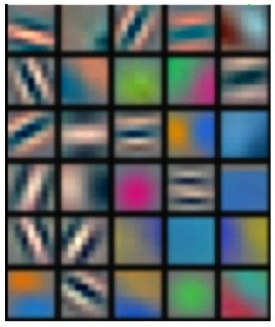
\includegraphics[width=\linewidth]{images/introduction/example_CNN_patterns}
		\caption{Example of simple patterns generated by a CNN.}
		%For more complex image:
		%The elaboration of an input image with deeper and deeper convolutional filters. The result are increasingly complicated patterns.
		\label{fig:example_CNN_patterns}
	\end{subfigure}
	\begin{subfigure}{0.7\textwidth}
		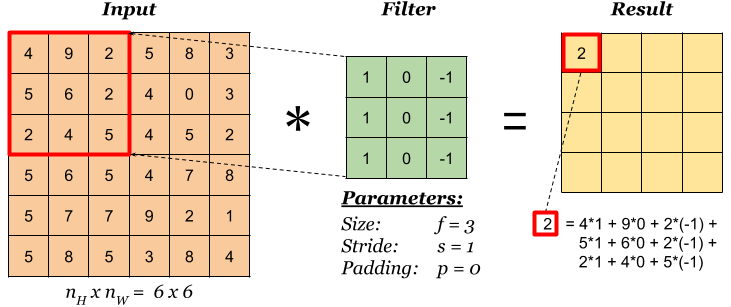
\includegraphics[width=\linewidth]{images/introduction/howItWorks_CNN}
		\captionsetup{margin=0.5cm}
		\caption{A numeric example of a convolution operation. The top-left, 3x3, section of the image is multiplied with a dot-product by the filter. The result is placed in the output matrix in the top-left corner.}
		\label{fig:howItWorks_CNN}
	\end{subfigure}
	\captionsetup{margin=0.5cm}
	\caption{The overall mechanics of a CNN.}
	\label{fig:CNN}
\end{figure}


\section{Structure of the thesis}
The next chapters are organized as follows. This section concludes the introduction (\Cref{cha:introduction}).\\
Then follow three chapters one for each main method: object detection in~\Cref{cha:detection}, object tracking in~\Cref{cha:tracking} and object recognition in~\Cref{cha:recognition}.\\
An overview of the entire algorithm and how it works together follow  in~\Cref{cha:solution}.\\
In the end, the conclusions are presented in~\Cref{cha:conclusions}.





